\documentclass{beamer}       % print frames
%\documentclass[notes=only]{beamer}   % only notes
%\documentclass{beamer}              % only frames
\newcounter{savedenum}
\newcommand*{\saveenum}{\setcounter{savedenum}{\theenumi}}
\newcommand*{\resume}{\setcounter{enumi}{\thesavedenum}}
\usepackage{multienum}
\usepackage[notocbib]{apacite}
    \renewcommand{\APACrefatitle}[2]{#1}
    \renewcommand{\APACrefbtitle}[2]{#1}
    \renewcommand{\APACrefbtitle}[2]{\Bem{#1}}
    \renewcommand{\APACrefaetitle}[2]{[#2]}
    \renewcommand{\APACrefbetitle}[2]{[#2]} 
\usepackage{textpos}
\usepackage{setspace}
\usepackage[T1]{fontenc}
\usefonttheme{serif}
%\usepackage{graphicx}
\usetheme{Boadilla}
\usepackage{hyperref}
\usepackage[UKenglish]{babel}
\usepackage{multicol}
\setcounter{tocdepth}{1} 
\usecolortheme{orchid}
\title[MOOD-Z, UZH]{Parsing and interrogating the Royal Society Corpus}
\author[Daniel McDonald]{Daniel McDonald}

\date{\today}

\begin{document}

\frame{\titlepage}

\begin{frame}
\frametitle{Introduction}

I've been parsing and interrogating the RSC. This means:

\begin{enumerate}
    \item Turning the \texttt{jstor bundle} into something that is parseable, but with retrievable metadata
    \item Experimenting with parsers
    \item Parsing everything, reintroduce metadata to parser output
    \item Developing tools: command interpreter, symbolic subcorpus management, automatic annotation, search filters
    \item Exploring the parsed corpus via lexicogrammatical querying
    \item (Trying to) generate some entropy\slash surprisal scores and methods
\end{enumerate}
\end{frame}

\begin{frame}
\frametitle{Preparing the corpus for parsing}

We can't just parse the XML right away, and we don't want to just strip out all that high-quality metadata. So:

\begin{enumerate}
    \item Make a version with and without metadata tags
    \item Add some metadata along the way using \texttt{langdetect}:
    \begin{itemize}
        \item Probable language
        \item Probability that text is English
    \end{itemize}
    \item Parse the version without metadata
    \item Use character offsets to add metadata to parser output
\end{enumerate}
The script for this is very quick to run, and can be improved or extended for future efforts.
\end{frame}

\begin{frame}
\frametitle{Things parsers don't like}

\begin{enumerate}
    \item Language\slash spelling change: noun\slash proper noun issues, \emph{hath}, etc.
    \item Text\slash metadata distinction
    \item Figures and tables as sentences
    \item Maths in text
    \item Non-English text
\end{enumerate}
\end{frame}

\begin{frame}[fragile]
\frametitle{Issue: text\slash metadata distinction}
\begin{verbatim}
IV. Part of a Letter from Mr James Yonge to Mr John Haughton, 
F. R. S. concerning the internal use of Cantharides. Plymouth, 
July 17. 1702. SIR, A Gentlewoman of 54 years old, who for a 
long time had been tormented with frequent Fits of the Stone
\end{verbatim}
\end{frame}

\begin{frame}[fragile]
\frametitle{Issue: figures, tables, references}
\footnotesize
\begin{verbatim}
13. Filix scandens Malab. pinnis integris alternatim sitis. 13 filix 
scandens Indica, ramulis ex adverso binis, foliis alternatim sitis, 
oblongis, angustis cuspidatis Ray V. 3. l. 3. p. 90. The top Leaf is 
often fork'd, the rest single. I have received it not only from fort St 
George, but also from the Grain and Gold Coasts of Guiney. 14. The Male 
Bangue. 14 Bange Clus. Exot 238. c. 25. & 290. c. 54. Fragos. 58. c. 26. 
Bangue arbor Cannabi similis ad omnia fere utilis seu Amsion (s. Opium) 
Linschot Ind. Or. pt. 4. c. 35. Bangue Cannabi simile I. B. Vol. 3. l. 
30. p. 449. c. 71. Cannabi similis exotica C. B. 320. 4. C. B. phyt. 
640. 
\end{verbatim}
\end{frame}

\begin{frame}[fragile]
\frametitle{Issue: maths}
\footnotesize
\begin{verbatim}
On the same principle we must proceed if such forms as cos (n log ), sin
(n log X), &c. are found in the second member. Ex. 3. Given s2 @ +d u 
+-=log ( ). Putting x=-g, we have D2u+eu=O. Make u=A+Bd, then on 
reducing D2A+2DB+ A+-(D2B+s-B-I)-0, whence, as in preceding examples, 
D2A+2DB+A = 0, D2B+-B= 1. This system of equations differs from those 
before considered, in that the second members do not both vanish. The 
fundamental theorem gives A==:am;, B=Zbm;, 1{ (mza+2mbmtI,)m } >2{ (mZbm
+b, _O'}= --l,1 6237whence m2aq+2mbm+aa_.l=O for all values of m, and 
m2bm+-b_-l=O for all values of m except m=0, which gives m2bm+-b _ I, or
b-=l; also from the other equation, a_-=O. From these, the values of am,
bm, corresponding to negative values only of n, may be determined; 
whence writing x for s, and solving the above equations relatively to 
a,_and b^_,, we have a*2 a,3 u=5a_+ a; a +&C. ++^+ + &c. +logx (b,+? + 
&C.) where a_=0, b=-i1; and in general a_ (m2am+2mb.), b_I= -m2bm. 
\end{verbatim}
\end{frame}

\begin{frame}[fragile]
\frametitle{Issue: Non-English}
\footnotesize
\begin{verbatim}
Verum priusquam ulterius progrediar hoc te monitum velim me usurpare 
illa quae demonstravit Clarissimus Newtonus in pag. 251, 252 & 253 
Princ. Phil. circa momentanea incrementa vel decrementa quantitatum quae 
fluxu continuo crescunt vel decrescunt, praesertim quod dignitatis 
cujuscunque A n/m momentum sit n/ma A n/m 1. Porro data fluxione n/m aA n
/m 1 vicissim reperiri potest quantitas fluens A n/m, 10 tollendo a de 
fluxione,20 fluxionis Indicem unitate augendo, 30 denique fluxionem 
dividendo per Indicem sic unitate auctum. Curvae abscissa designabitur 
deinceps per x, ejus fluxio per x, ordinatim applicata per y, ejusque 
fluxio per y His positis ut ad quadraturas deveniamus, 10 assumatur 
valor ordinatim applicatae ope aequationis naturam Curvae exprimentis. 
20 Multiplicetur hic valor 
\end{verbatim}
\end{frame}

\begin{frame}\frametitle{Solutions}
    Ways to solve these problems for the investigation of the RSC:
    \begin{enumerate}
        \item Via pre-processing:
        \begin{itemize}
            \item Searching, manual\slash semi automatic correction
            \item Time consuming and expensive, but can create high quality resources
        \end{itemize}
        \item Via post-processing:
    \begin{itemize}
        \item Use language identification metadata to filter corpus during search
        \item Exclude based on lexicogrammatical criteria
        \item Fast, but sacrifices data
    \end{itemize}
    \item Iterative development: back and forth between the two (yes!)
    \end{enumerate}
\end{frame}

\begin{frame}
\frametitle{Parsing possibilities}
\begin{itemize}
    \item A lot of messy data, so speed and accuracy are both issues
    \item Faster parsers provide less, and are less accurate
    \item \texttt{spaCy}: no constituency, no coreference resolution, no \texttt{copula=head}
    \item \texttt{CoreNLP}: slower, Java trickiness
    \item The ideal solution would include:
    \begin{itemize}
        \item Cleaner data 
        \item Using the best POS tagging info in the model
        \item training a model from corrected parser output
        \item training multiple models for different time periods
    \end{itemize}
\end{itemize}

\end{frame}

\begin{frame}
\frametitle{Parsing}
\begin{enumerate}
    \item Using \texttt{CoreNLP} (via \texttt{corpkit})
    \begin{itemize}
        \item Provides lemmatisation, POS, NER, constituency, typed dependency, coreference resolution
        \item Coreference resolution is slow, memory intensive, inaccurate, causes a few big errors
    \end{itemize}
    \item Great example of an \emph{embarrassingly parallel} job
    \item Parsing time unknown---a few days with 15 processes, some Java errors
\end{enumerate}
\end{frame}


\begin{frame}
    \frametitle{The good}
    \centering
    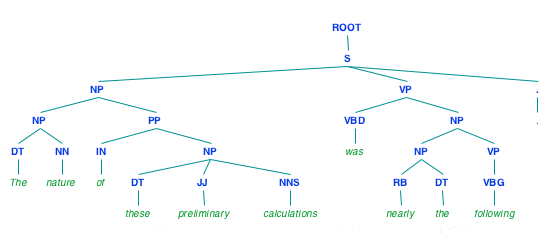
\includegraphics[width=0.90\textwidth]{../images/good}
\end{frame}

\begin{frame}
    \frametitle{The bad}
    \centering
    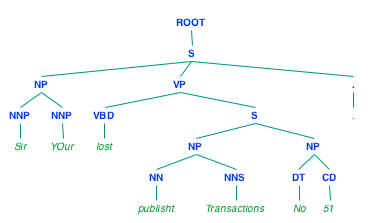
\includegraphics[width=0.90\textwidth]{../images/bad}
\end{frame}

\begin{frame}
    \frametitle{The ugly}
    \centering
    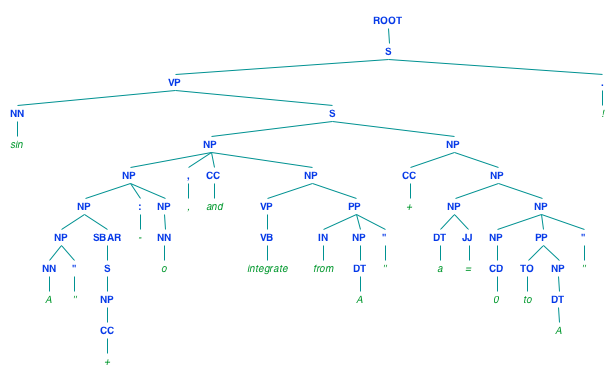
\includegraphics[width=0.90\textwidth]{../images/ugly}
\end{frame}



\begin{frame}
\frametitle{\texttt{corpkit}: tool for analysis}

\texttt{corpkit} is my module for making and querying parsed corpora.

\begin{enumerate}
    \item Traverse and output grammatical annotations and metadata
    \item Interrogate and concordance at the same time---use concordance to identify\slash remove false positives, do thematic categorisation, and then recalculate results
    \item Language models including grammatical information (beta)
    \item Fast, cross platform, open source, documented, version control 
    \item Interfaces: Python API, GUI, and more recent \textbf{CQP-style interpreter}
\end{enumerate}
\end{frame}

\begin{frame}
\frametitle{Tool extensions}

Some feedback on \texttt{corpkit} led to:

\begin{enumerate}
    \item Metadata as subcorpora and filter
    \item Symbolic and multi-level subcorpora
    \item Semi-automatic annotation via concordancing
    \item Fully scriptable
\end{enumerate}
\end{frame}

\begin{frame}
\frametitle{\texttt{corpkit interpreter demo}}

\url{http://corpkit.readthedocs.io}

\end{frame}

\begin{frame}
\frametitle{RSC: interrogation}

The strategy:

\begin{itemize}
    \item Use years as subcorpora
    \item Search for sentences whose root lemma is in VerbNet
    \item Tag these sentences and filter out the others
    \item Filter out texts (not sentences, yet) that are not English
    \item Get general features, and use these to generate relative frequencies for more specific phenomena
    \item Automate the process of discovering longitudinal change
    \item Keep everything logged, saved, and on GitHub
\end{itemize}
\end{frame}

\begin{frame}
    \frametitle{Derived features}
    \centering
    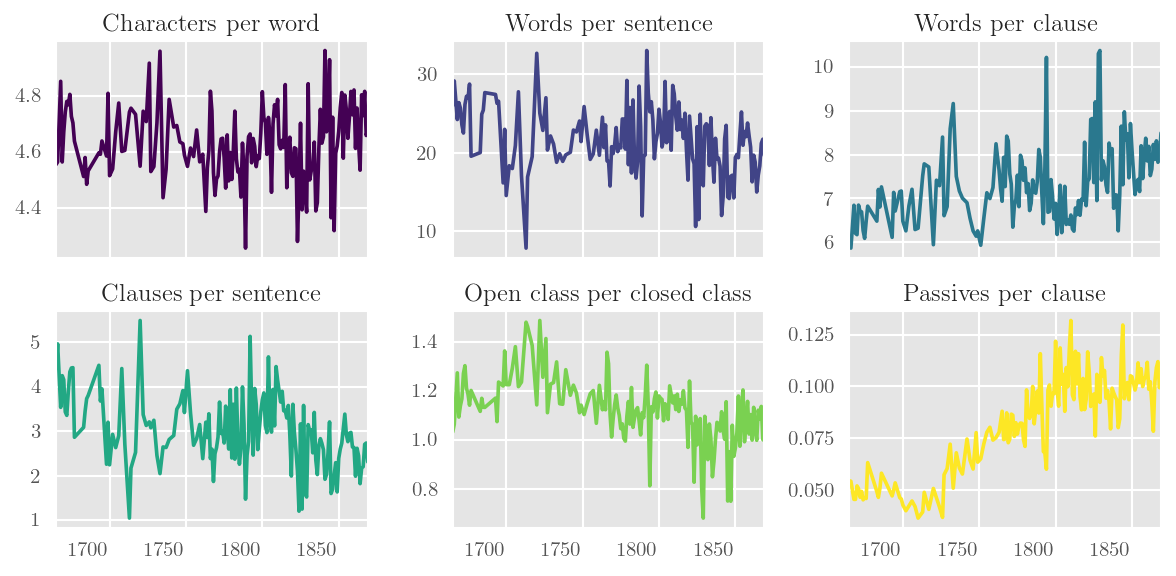
\includegraphics[width=0.90\textwidth]{../images/best-derived}
\end{frame}

\begin{frame}
    \frametitle{POS tag and parser accuracy}
    \centering
    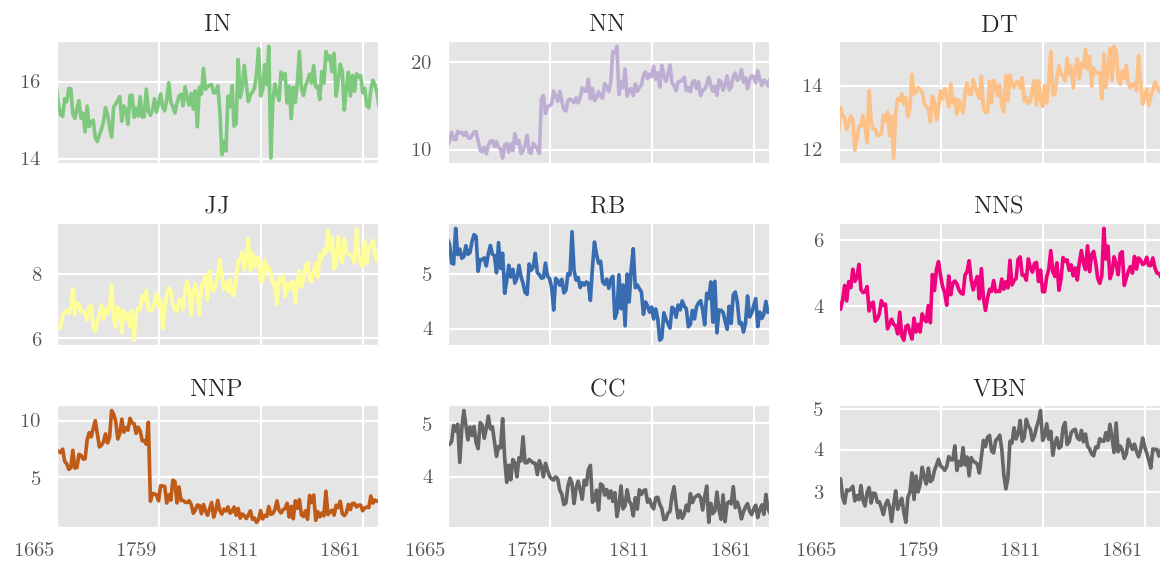
\includegraphics[width=0.90\textwidth]{../images/postag}
\end{frame}

\begin{frame}
    \frametitle{Wordclass and parser accuracy}
    \centering
    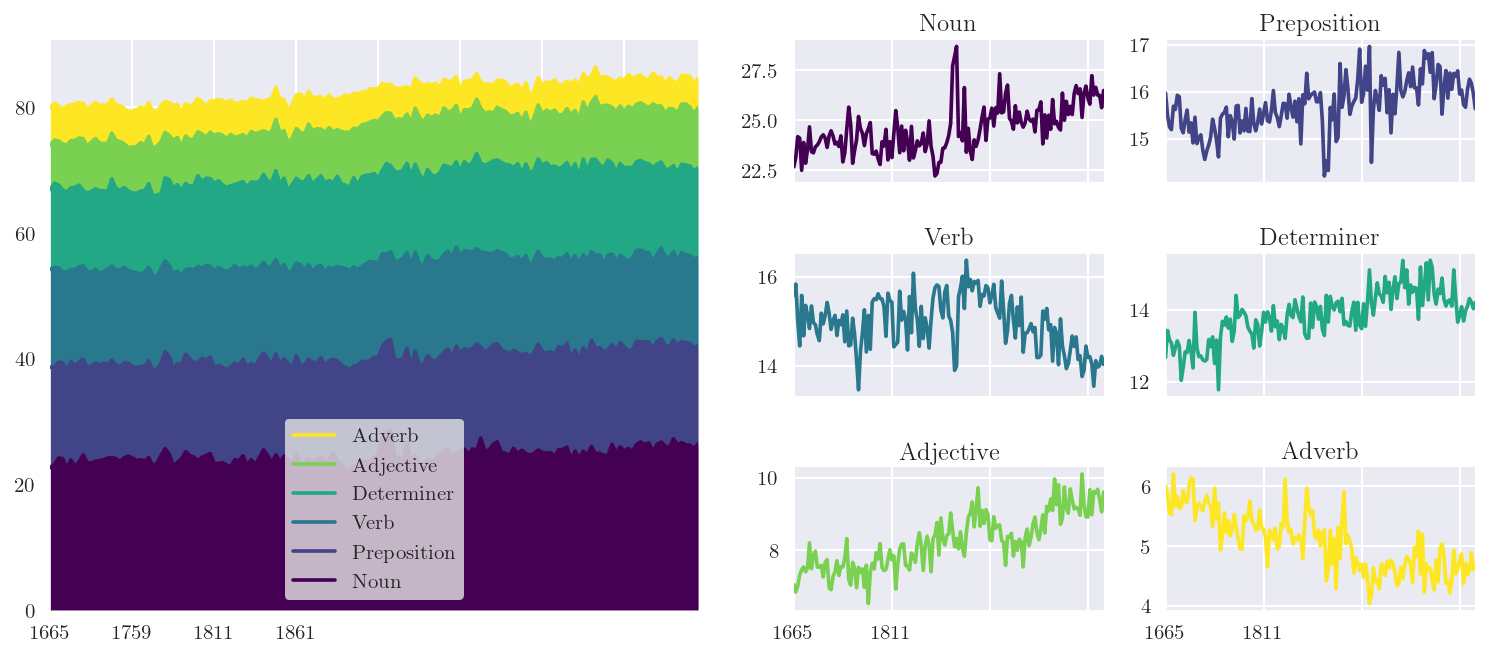
\includegraphics[width=0.90\textwidth]{../images/multi-wc}
\end{frame}

\begin{frame}
    \frametitle{Mixing wordclass and dep type}
    \centering
    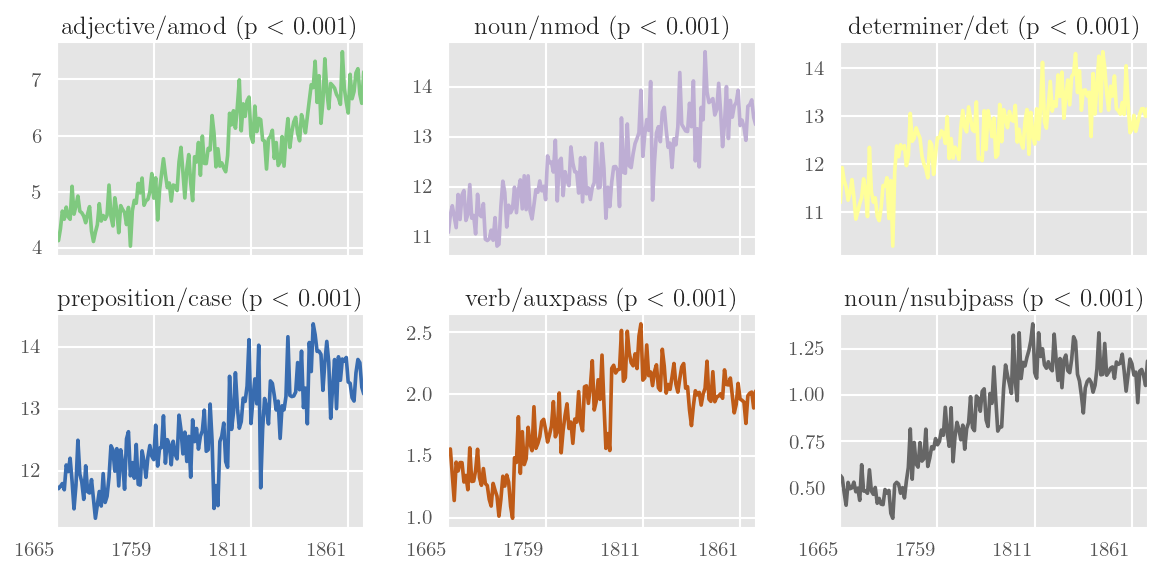
\includegraphics[width=0.90\textwidth]{../images/6-inc}
\end{frame}

\begin{frame}
    \frametitle{Mixing wordclass and dep type}
    \centering
    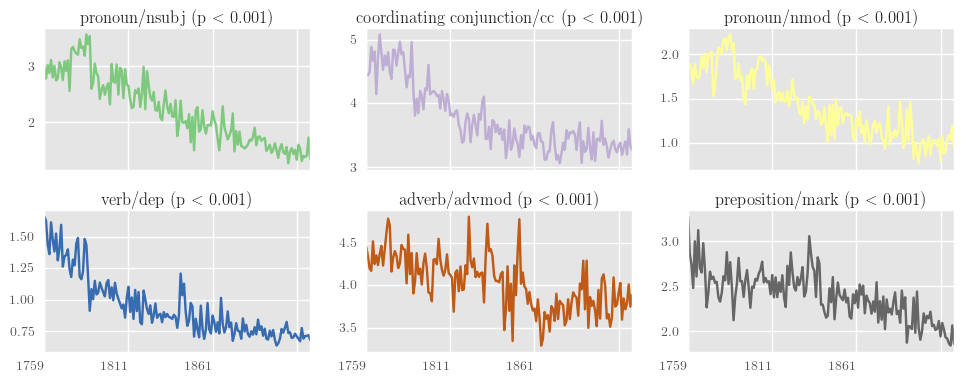
\includegraphics[width=0.90\textwidth]{../images/6-dec}
\end{frame}

\begin{frame}
    \frametitle{Increasingly frequent participants}
    \centering
    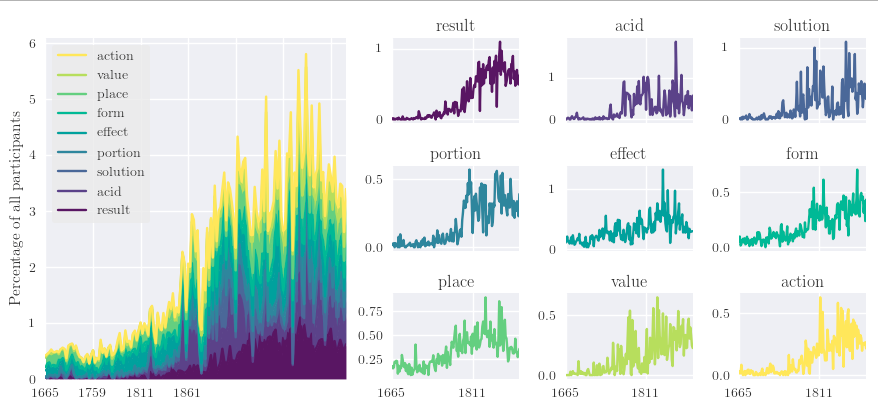
\includegraphics[width=0.90\textwidth]{../images/inc-part}
\end{frame}

\begin{frame}
    \frametitle{Decreasingly frequent participants}
    \centering
    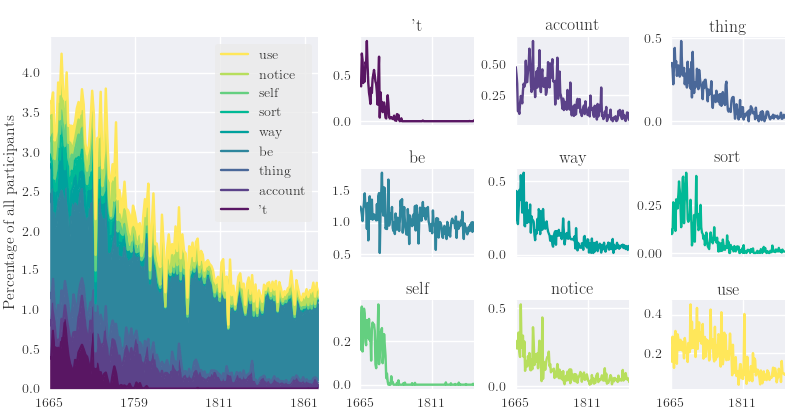
\includegraphics[width=0.90\textwidth]{../images/dec-part}
\end{frame}

\begin{frame}
    \frametitle{Increasingly frequent processes}
    \centering
    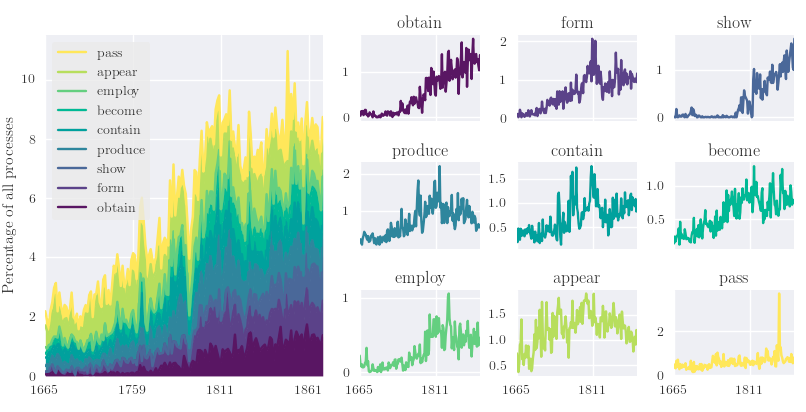
\includegraphics[width=0.90\textwidth]{../images/inc-proc}
\end{frame}

\begin{frame}
    \frametitle{Decreasingly frequent processes}
    \centering
    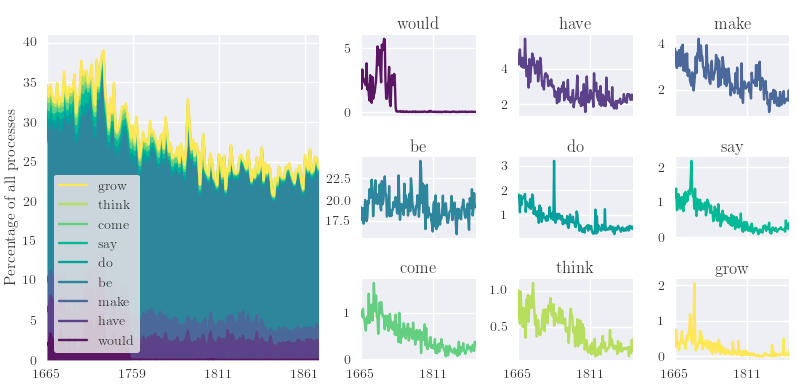
\includegraphics[width=0.90\textwidth]{../images/dec-proc}
\end{frame}

\begin{frame}
\frametitle{Discussion}
\begin{enumerate}
    \item Parsing will need to be repeated reliably as the corpus is improved
    \item To what extent will this approach model parser accuracy rather than language change?
    \item Parser accuracy \emph{as} language change
\end{enumerate}
\end{frame}

\begin{frame}
\frametitle{Next steps}

\begin{enumerate}
    \item Use the annotations to get bad text in the original bundle
    \item Use tool for syntactic language models?
    \item Measure parser accuracy
    \item Word\slash sentence\slash text level annotations for entropy?
    \item What should the training data be? The corpus? Subcorpus? Training set from (groups of) subcorpora?
\end{enumerate}
\end{frame}

\end{document}